%\documentclass[handout]{ximera}
\documentclass[nooutcomes]{ximera}

\usepackage{gensymb}
\usepackage{tabularx}
\usepackage{mdframed}
\usepackage{pdfpages}
%\usepackage{chngcntr}

\let\problem\relax
\let\endproblem\relax

\newcommand{\property}[2]{#1#2}




\newtheoremstyle{SlantTheorem}{\topsep}{\fill}%%% space between body and thm
 {\slshape}                      %%% Thm body font
 {}                              %%% Indent amount (empty = no indent)
 {\bfseries\sffamily}            %%% Thm head font
 {}                              %%% Punctuation after thm head
 {3ex}                           %%% Space after thm head
 {\thmname{#1}\thmnumber{ #2}\thmnote{ \bfseries(#3)}} %%% Thm head spec
\theoremstyle{SlantTheorem}
\newtheorem{problem}{Problem}[]

%\counterwithin*{problem}{section}



%%%%%%%%%%%%%%%%%%%%%%%%%%%%Jenny's code%%%%%%%%%%%%%%%%%%%%

%%% Solution environment
%\newenvironment{solution}{
%\ifhandout\setbox0\vbox\bgroup\else
%\begin{trivlist}\item[\hskip \labelsep\small\itshape\bfseries Solution\hspace{2ex}]
%\par\noindent\upshape\small
%\fi}
%{\ifhandout\egroup\else
%\end{trivlist}
%\fi}
%
%
%%% instructorIntro environment
%\ifhandout
%\newenvironment{instructorIntro}[1][false]%
%{%
%\def\givenatend{\boolean{#1}}\ifthenelse{\boolean{#1}}{\begin{trivlist}\item}{\setbox0\vbox\bgroup}{}
%}
%{%
%\ifthenelse{\givenatend}{\end{trivlist}}{\egroup}{}
%}
%\else
%\newenvironment{instructorIntro}[1][false]%
%{%
%  \ifthenelse{\boolean{#1}}{\begin{trivlist}\item[\hskip \labelsep\bfseries Instructor Notes:\hspace{2ex}]}
%{\begin{trivlist}\item[\hskip \labelsep\bfseries Instructor Notes:\hspace{2ex}]}
%{}
%}
%% %% line at the bottom} 
%{\end{trivlist}\par\addvspace{.5ex}\nobreak\noindent\hung} 
%\fi
%
%


\let\instructorNotes\relax
\let\endinstructorNotes\relax
%%% instructorNotes environment
\ifhandout
\newenvironment{instructorNotes}[1][false]%
{%
\def\givenatend{\boolean{#1}}\ifthenelse{\boolean{#1}}{\begin{trivlist}\item}{\setbox0\vbox\bgroup}{}
}
{%
\ifthenelse{\givenatend}{\end{trivlist}}{\egroup}{}
}
\else
\newenvironment{instructorNotes}[1][false]%
{%
  \ifthenelse{\boolean{#1}}{\begin{trivlist}\item[\hskip \labelsep\bfseries {\Large Instructor Notes: \\} \hspace{\textwidth} ]}
{\begin{trivlist}\item[\hskip \labelsep\bfseries {\Large Instructor Notes: \\} \hspace{\textwidth} ]}
{}
}
{\end{trivlist}}
\fi


%% Suggested Timing
\newcommand{\timing}[1]{{\bf Suggested Timing: \hspace{2ex}} #1}




\hypersetup{
    colorlinks=true,       % false: boxed links; true: colored links
    linkcolor=blue,          % color of internal links (change box color with linkbordercolor)
    citecolor=green,        % color of links to bibliography
    filecolor=magenta,      % color of file links
    urlcolor=cyan           % color of external links
}

\title{Pythagorean Theorem}
\author{Bart Snapp and Brad Findell}

\outcome{Learning outcome goes here.}

\begin{document}
\begin{abstract}
  We prove the most famous theorem of all, the Pythagorean Theorem.
\end{abstract}
\maketitle

\begin{teachingnote}
Before problem 1, ask:  ``State the Pythagorean Theorem.''  Give students about a minute to write something down.  Many students will write only, ``$a^2 + b^2 = c^2$.''  Then in whole class discussion, draw out the missing pieces:  (1) that $a$, $b$, and $c$ are side lengths of a triangle;  (2) that the triangle is a right triangle; and (3) that $c$ is the length of the hypotenuse.  Then, the class decision can be as follows: 
 
\begin{quote}\textbf{Pythagorean Theorem:}  Suppose a triangle has side lengths $a$, $b$, and $c$.  If the triangle is right with hypotenuse $c$, then $a^2 + b^2 = c^2$. 
\end{quote}
The advantage of this phrasing is that it paves the way for a clear statement of a converse (below).   

Some students will use only the left picture and algebra (i.e., the distributive property) to get the desired result.  The advantage of both pictures is that algebra is not necessary, as the right picture provides the distributive property via rearranging the pieces.  

Once they have proven the Pythagorean Theorem for the particular triangle as drawn, ask, ``How do we know it will work for any triangle?''  The conceptual leap is that the reasoning is exactly the same.  

The term \emph{converse} may need to be introduced.  Perhaps include an example of a true statement with a false converse (e.g., about vertical angles, or about divisibility by 4 and even).  

\begin{quote}
\textbf{Converse of the Pythagorean Theorem:}  Suppose a triangle has side lengths $a$, $b$, and $c$.  If $a^2 + b^2 = c^2$, then the triangle is right with hypotenuse $c$. 
\end{quote}

For the proof, construct a separate right triangle with legs of length $a$ and $b$ and hypotenuse $d$.  By the (forward direction) of the Pythagorean Theorem, $a^2+b^2=d^2$.  (For students who find it difficult to accept this reasoning, it can help to remind them that a statement and its converse are logically distinct.)  By algebra, $c=d$.  By SSS, the two triangles are congruent, so the original triangle must be right.  

Perhaps add a problem about the history involving Egyptians, ropes, knots, and right angles.  Ask whether it is about the theorem or the converse. 
\end{teachingnote}


\begin{problem}
Give two explanations of how the following picture ``proves''
  the Pythagorean Theorem, one using algebra and one without 
  algebra.\margincomment{CCSS 8.G.6. Explain a proof of the 
  Pythagorean Theorem and its converse.}
\begin{image}
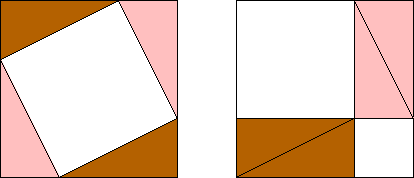
\includegraphics[scale=1.3]{pbppyth1.pdf}
\end{image}
\end{problem}

\begin{problem}
State the converse of the Pythagorean Theorem and prove it.  
\end{problem}

\end{document}

